Pour $t >> \tau, \begin{array}{rcl}
e^{-\frac{t}{\tau}} &\rightarrow& 0 \\
(\frac{t}{\tau})-1 &\rightarrow& \frac{t}{\tau}
\end{array}$ D'où ~\\
\begin{center}\fbox{$z(t) \simeq h-gt\tau $}\end{center}
D'où le mouvement uniforme rectiligne pour $t >> \tau$

\paragraph{Rappels}
\begin{itemize}
\item Mouvement rectiligne uniformément accéléré : $\vec{F} \overrightarrow{Constante}$
\item Mouvement rectiligne amortie : F dépend de la fonction de la vitesse, et des frottements visqueux / fluide
\end{itemize}

\subsection{Lancé oblique d'un projectile}

\begin{wrapfigure}[8]{r}{0pt}
	\begin{tikzpicture}
		\draw[->] (0, 0) -- (2, 0) node [right] {x};
		\draw[->] (0, 0) -- (0, 2) node[above] {z};
		\draw[->] (0, 0) -- (-0.5, -1.0.5) node[below left]{y};
		\draw[red, ->] (0, 0) -- (0.2, 0) node[below]{$\vec{i}$};
		\draw[red, ->] (0, 0) -- (0, 0.2) node[below]{$\vec{k}$};
		\draw[red, ->] (0, 0) -- (-0.2, -0.2) node[below]{$\vec{j}$};
		\draw[blue] (0, 0) .. controls (0.7, 1.5) and (1.7, 1.5) .. (2, 0);
		\draw[thick, green, ->] (0, 0) -- (45:1cm) node [above] {$\vec{v_0}$};
		\draw[blue, ->] (0.3, 0) arc (0:45:0.3) node [right] {$\alpha$};
		\draw[red, dashed] (0, 0) -- (1.7, 1.7) node [above right] {$y$};
		\draw[fill=black] (0, 0) circle (0.05) node [below] {$m$};
	\end{tikzpicture}
\end{wrapfigure}

\begin{itemize}
	\item m ponctuelle
	\item lancé avec $\vec{v} = \vec{v_0}$
	\item On néglige les forces de frottement avec l'air ainsi que la poussé d'archimède
	\item bilan des forces: \[\vec{P} = m \vec{g} = m \cdot g \cdot \vec{k}\]
	\item PFD : $m\vec{a} = \vec{P} = -mg\vec{k}$
\end{itemize}

\[\left\{
		\begin{array}{rcl}
			m\ddot{x} &=& 0 \\
			m\ddot{y} &=& 0 \\
			m\ddot{z} &=& -mg \\
		\end{array}\right.
		\left\{
		\begin{array}{rcl}
			\dot{x} &=& C_x \\
			\dot{y} &=& C_y \\
			\dot{z} &=& -gt + C_z \\
		\end{array}\right.
	\]
	\[\text{À } t=0 , v(0) = v_0 ~\\
	\text{Composantes sur x, z: } ~\\
	\text{A } t = 0 \left\{
		\begin{array}{rcl}
			v_x &=& v_0 \cos(\alpha) \\
			v_z &=& v_0 \sin(\alpha) \\
			v_y &=& 0 \end{array} \right.
			\text{D'où } 
		\left\{
		\begin{array}{rcl}
				C_x &=& v_0 \cos(\alpha) \\
				C_y &=& 0 \\
				C_z &=& v_0 \sin(\alpha) \end{array}\right. ~\\
		\left\{ \begin{array}{rcl}
				\dot{x} &=& v_0 \cos (\alpha) \\
				\dot{y} &=& 0 \\
				\dot{z} &=& -gt + v_0 \sin(\alpha) \end{array}\right. ~\\
		\vec{v}(t) = v_0\cos(\alpha)\vec{i} + (-gt+v_0\sin(\alpha))\vec{k}\] 

\[\begin{array}{rcl}
		\overrightarrow{OM} &=& x(t)\vec{i} + y(t) \vec{j} + z(t) \vec{k} \\
		x(t) &=& v_0\cos(\alpha) \cdot + C'_x \\
		y(t) &=& C'_y = 0 \\
z(t) &=& -\frac{1}{2}gt^2 + v_0 \sin(\alpha)\cdot t + C'_z \end{array}\]

		\[\text{À } t=0,
			\left\{ \begin{array}{rcl}
			x &=& 0 \\
			y &=& 0 \\
			z &=& 0 \\
			z &=& 0\end{array}\right.\]

		\[\left\{\begin{array}{rcl}
			C'_x &=& 0 \\
			C'_y &=& 0 \\
			C'_z &=& 0 \end{array}\right.\]

D'où un mouvement uniforme par rapport à $Ox$, et un mouvement uniforme accéléré par rapport à $Oz$.
Le mouvement est dans le plan de $\vec{v_0}$ car par de $\vec{F} \perp  \vec{v_0}$

\paragraph{Équation de la trajectoire $z(x)$ }

\[\begin{array}{rclr}
		x(t) &=& v_0 \cos(\alpha) t & (1) \\
z(t) &=& -\frac{1}{2}gt^2 + v_0 \sin(\alpha)\cdot & (2)\end{array}\]
	
	Ce qui donne : $t = \frac{x}{v_0\cos(\alpha)} \Rightarrow z=-\frac{1}{2}g\frac{x^2}{v_0^2\cos(\alpha)^2} + v_0 \sin(\alpha) \cdot \frac{x}{v_0\cos(\alpha)}$ ~\\ ~\\
\begin{center} D'où \fbox{$z(x) = x-(\frac{g}{2v_0^2 \cos(\alpha)^2}x + \tan(\alpha))$}\end{center}

	Ceci est : \begin{itemize}
		\item Un équation d'une parabole 
		\item Passant par : $(x,z) = (0, 0)$
	\end{itemize}
	
	\begin{center} Pour $z=0$, \fbox{$\begin{array}{rclr}
		x_p &=& 2\sin(\alpha) \cos(\alpha) \frac{V_0^2}{g} \\
	x_p &=& \sin(2\alpha) \frac{v_0^2}{g} & \text{ Donne la portée maximal} \end{array}$}\end{center}

	La portée est maximal pour $\sin(2\alpha) = 1$ donc pour $\alpha = \frac{\pi}{4}$

	\paragraph{Hauteur maximal}
	Elle est maximal pour $z'(x) = 0$ et, comme la trajectoire est une parabole, elle est symétrique par une droite parallèle à $O_z$ passant par $\frac{x_p}{2}$
	\[z(\frac{x_p}{2}) = \text{ hauteur }\] 

	\subsection{Oscillateurs harmoniques}

	\begin{wrapfigure}[6]{r}{0pt}
		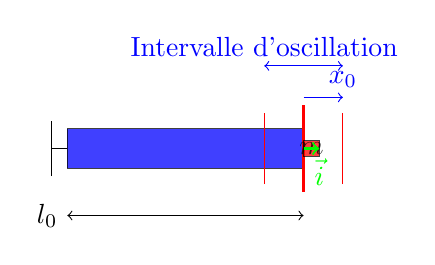
\begin{tikzpicture}[rotate=90]
			\draw[fill=blue, opacity=0.75] (0, 0) rectangle (0.5, 3);
			\draw[] (0.25, 3) --+ (0, 0.2);
			\draw[] (-0.1, 3.2) -- (0.6, 3.2);
			\draw[thick, red] (-0.3, 0) -- (0.8, 0);
			\draw[blue, <->] (1.3, -0.5) -- (1.3, 0.5) node[align=center, above] {Intervalle d'oscillation};
			\draw[red, thin] (-0.2, -0.5) -- (0.7, -0.5);
			\draw[red, thin] (-0.2, 0.5) -- (0.7, 0.5);
			\draw[blue, ->] (0.9, 0) -- (0.9, -0.5) node [above] {$x_0$};
			\draw[<->] (-0.6, 0) -- (-0.6, 3) node [left] {$l_0$};
			\draw[fill=red, opacity=0.75] (0.15, 0) rectangle (0.35, -0.2) node [midway] {$m$};
			\draw[->, green, thick] (0.25, 0) -- (0.25, -0.2) node [below] {$\vec{i}$};
		\end{tikzpicture}
	\end{wrapfigure}

	\ul{System} : \begin{itemize}
		\item masse m
		\item Ressort de raideur k et de longueur $l_0$ 
		\item t=0, on déforme de $x_0$
		\item On néglige les frottements et le poids du ressort
		\item Bilan de forces : $\vec{P}$ et $\vec{R}$ s'équilibre car abscence de frottements.
		\item $\vec{F} = -k(l-l_0)\vec{i} = -kx(t)\vec{i}$
		\item PFD : $m\vec{a} = \vec{F} = -kx\vec{i}$
	\end{itemize}

	\paragraph{Projection sur $O_x$}
	\begin{center}
		\fbox{$m\ddot{x} = -kx$}
		\fbox{$\ddot{x} + \frac{k}{m}\vec{i} = 0$}
	\end{center}

	On pose $\frac{k}{m}=\omega^2$ : \[\ddot{x}(t) + \omega^2 x(t) = 0\]
	La fonction sinusoïdale est celle dont la dérivée second est le produit de cette fonction par une constante. ~\\
	La solution générale est de la forme \fbox{$x(t) = A \cos(\omaga t) + B\sin(\omaga t)$} ~\\
	La vitesse : $\dot{x} = -A\omega \sin(\omega) t + B\omega \cos(\omega) t$

	Pour déterminer A et B, on regarde les conditions initiales:
	\[\left\{\begin{array}{rcl}
				x(0) &=& 0 \\
				\dot{x} &=& 0
		\end{array}\right.
	\Rightarrow 
	\left\{\begin{array}{rcl}
		x(0) &=& A = x_0 \\
		\dot{x}(0) &=& B\omega \Rightarrow B=0\end{array}\right.
			\text{D'ou } \left\{
			\begin{array}{rcl}
			x(t) &=& x_0\cos(\omaga t) \\
		\dot{x}(t) &=& -x_0\omega\sin(\omaga t) \end{array}\right.\]
